\documentclass[default]{aastex702}

\shorttitle{TIC 31065777 Eclipse Candidate}
\shortauthors{Barrientos}
\submitjournal{RNAAS}

\begin{document}

\title{Raw-pixel Validation of a 40.5717-day Eclipse Candidate Associated with TIC 31065777}

\author[gname=Henry,sname=Barrientos]{Henry Barrientos}
\affiliation{Independent Researcher, Collinsville, OK 74021, USA}
\email[show]{henrywaynebarrientos@gmail.com}

\begin{abstract}
I report raw-pixel validation of five eclipse-like events associated with TIC 31065777 in public Transiting Exoplanet Survey Satellite observations. The target appears in the unvetted, unvalidated supplement to the TESS Ten Thousand Catalog but not in its validated eclipsing-binary sample. Events in Sectors 8, 9, 35, 36, and 89 follow a linear ephemeris with period $40.5717302 \pm 0.0000688$ days. A 1.5-pixel aperture gives a median fitted depth of 6.207\%, and a joint trapezoid fit gives a duration of $2.920 \pm 0.041$ hr. Period estimates are stable across aperture sizes and leave-one-sector-out tests. Missing-light centroids fall 0.16--0.51 TESS pixel from the catalog position. The data support an ordinary eclipsing companion or unresolved blended system; photometry alone does not establish the companion class.
\end{abstract}

\section{Analysis}

The Transiting Exoplanet Survey Satellite (TESS; \citealt{ricker2015}) observed TIC 31065777 at R.A. $=135.070042\arcdeg$, decl. $=-45.052218\arcdeg$ in multiple sectors. I encountered the target during an exploratory search of public MIT Quick-Look Pipeline (QLP; \citealt{huang2020}) light curves. A subsequent exact-TIC cross-match found the source in Table 2, the unvetted and unvalidated machine-learning candidate list of \citet{kostov2025}, but not in their Tables 3 or 4 of validated new or previously known eclipsing binaries. The analysis here tests that candidate at the pixel level and incorporates the later Sector 89 observation.

I downloaded 15 by 15 pixel TESSCut products from the Mikulski Archive for Space Telescopes for Sectors 8, 9, 35, 36, and 89. I retained finite, quality-zero cadences and subtracted each cadence's median border-pixel background. Circular apertures of radii 1.0, 1.5, 2.0, and 2.5 pixels were centered on the TESS Input Catalog position \citep{stassun2019}. Within 0.55 days of each expected event, I divided the aperture sum by its local out-of-event median. A joint least-squares trapezoid model used a shared epoch, period, duration, and ingress fraction, with a separate depth, baseline, and linear trend for each sector. I then refit event centers at a fixed joint shape and fit their cycle numbers $N=(0,1,18,19,54)$ with
\begin{equation}
T_N = 1527.534962(337) + N\,40.571730224(688)\ {\rm BTJD},
\end{equation}
where BTJD is BJD $-2457000$ and parentheses give the uncertainty in the final digits.

\section{Validation and Interpretation}

The five 1.5-pixel-aperture depths span 5.973\%--6.663\%, with median 6.207\% (Figure~\ref{fig:validation}). The joint duration is $2.9198 \pm 0.0408$ hr. Across the four aperture radii, fitted periods span only 1.61 s. Leaving out each sector in turn predicts the omitted event to within 1.90 minutes; a 2000-trial parametric bootstrap of event-center errors gives a 95\% period interval of 40.57160--40.57187 days. These uncertainties propagate measured event-center errors and do not constitute a blind-search false-alarm probability because the target and events were selected after inspecting the data.

Four blank apertures offset by four pixels show maximum absolute apparent depths of 0.10\%--0.94\%, and target-aperture windows shifted by one or two days reach 0.34\%, all below the 6.2\% event signal. Difference-image missing-light centroids are 0.16--0.51 TESS pixel from the target position, and every sector passes the same quality, coherence, timing, and greater-than-$5\sigma$ localization-depth criteria. This reduces resolved-background and time-localized instrumental explanations, but a TESS pixel is approximately $21\arcsec$ \citep{ricker2015}; unresolved blending remains possible.

The measurements therefore support a recurring eclipse candidate associated with the TIC 31065777 aperture. They do not demonstrate a planet, determine a companion mass, or fully identify the eclipsed source. Multicolor time-series photometry at higher angular resolution can test chromaticity and blending, while spectroscopy can determine whether the system is a stellar binary. Code, derived tables, source-product hashes, and an executable evidence packet accompany this Note.

\begin{figure}[ht!]
\centering
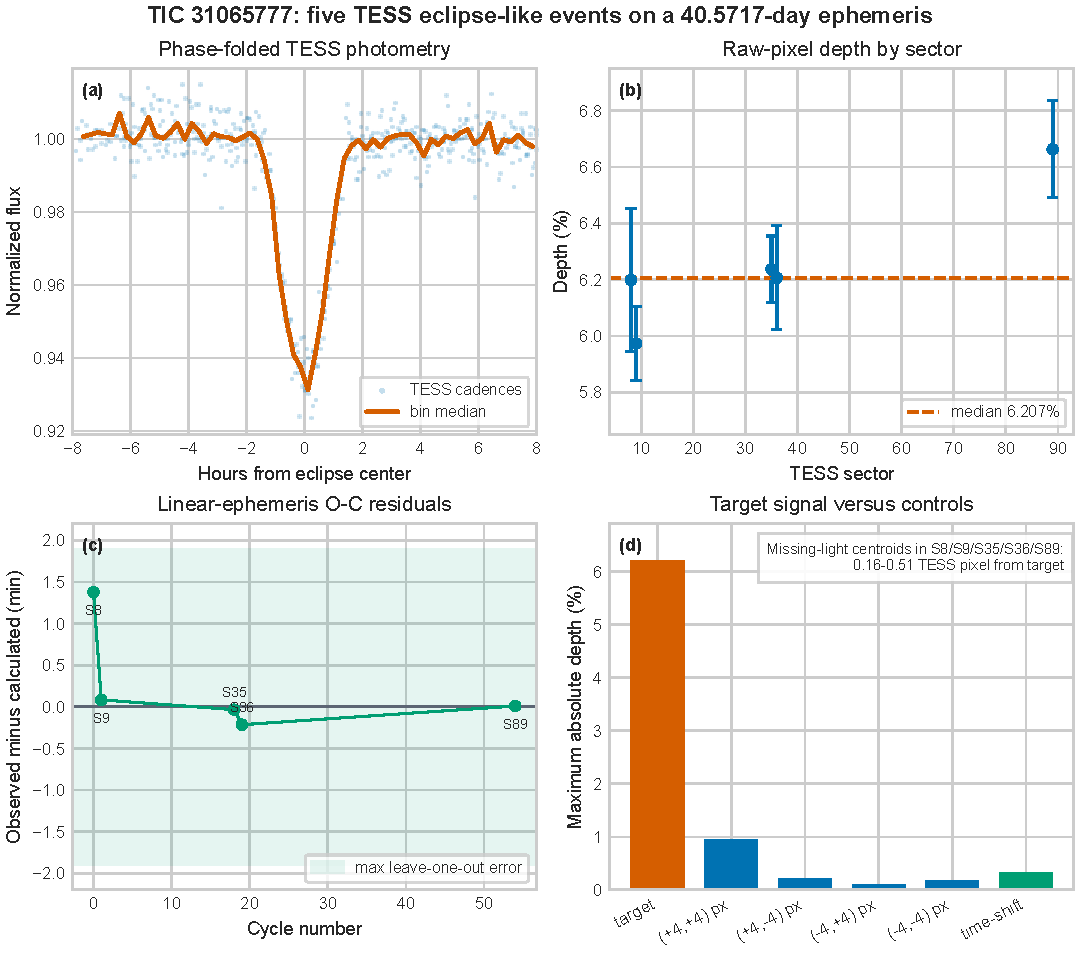
\includegraphics[width=\textwidth]{TIC_31065777_RNAAS_FIGURE.pdf}
\caption{Five-event photometric validation of TIC 31065777. (a) Individual phase-folded TESS cadences (light blue) and bin medians (orange). (b) Fitted 1.5-pixel-aperture depths with $1\sigma$ errors; the dashed line is their median. (c) Observed-minus-calculated event-center residuals; the shaded band marks the largest leave-one-sector-out prediction error. (d) Target median depth compared with the maximum absolute signal at four blank apertures and at time-shifted target windows. The annotation gives missing-light centroid separations.\label{fig:validation}}
\end{figure}

\begin{acknowledgments}
This paper includes data collected by the TESS mission and obtained from the MAST data archive at the Space Telescope Science Institute. Funding for the TESS mission is provided by NASA's Science Mission Directorate. I used the public MIT QLP high-level science products. I used OpenAI Codex to assist with code review, reproducibility checks, and manuscript drafting; I inspected the outputs, reran the analysis, and accept responsibility for the submitted work \citep{openai2026,vishniac2023}.
\end{acknowledgments}

\facility{TESS}

\software{Astropy \citep{astropy2022}, Lightkurve \citep{lightkurve2018}, NumPy, pandas, SciPy, Matplotlib}

\bibliographystyle{aasjournalv7.1}
\bibliography{references}

\end{document}
